% --------------------------------------------------------------------------
% -- Introduction --
% \acresetall  % Use this if you want acronyms to be fully stated upon first use again, such as in new chapters
As any nation prepares to meet their respective demands for energy, they are faced with the challenge of addressing four major issues. First, the sources of energy production must produce sufficient energy to reliably meet the demands of growing populations and economies. Second, the serious threat of climate change and air pollution due to emissions demands alternatives that can fuel economic growth while minimizing damage to the planet. Third, the sources of energy must be flexible enough to respond to seasonal and hourly fluctuations in demand. Finally, all of the above objectives must be met through economically viable combinations of energy sources that are affordable.
No one source of energy has optimized all four of these objectives. Coal-fired energy has fueled the economic growth of most developed nations, producing vast amounts of energy and creating a reliable grid for distributing that energy. But the environmental and safety costs of coal have been enormous, which has led to the search for viable alternatives. Natural gas, the primary affordable alternative in the United States, has less particulate pollution but still produces greenhouse gas emissions. Natural gas power plants, unlike most nuclear and coal power plants in the United States, were built with flexibility in mind and are the typical load following means of energy production \cite{MITEnergyInitiative2011}. Renewable sources - such as solar, wind and hydro - have grown significantly, but their capacity to generate sufficient energy and respond to fluctuating demand have limited their utility. Nuclear power is low-emitting and reliable, but its affordability and flexibility are issues to address.

Various ways of integrating non-emitting sources of power; such as solar, wind, and nuclear, provide approaches to addressing the four objectives listed above - reducing greenhouse gas emissions while increasing grid reliability and flexibility. Three ways to achieve greater flexibility without sacrificing reliability include: 1) more flexible production to load follow as with natural gas; 2) greater storage capacity provided through chemical and thermal of batteries; and 3)  allocation strategies that direct excess heat or electricity to an industrial process when the grid has lower demand. \ac{nrhess} focus on the third strategy to create a reliable, flexible system while seeking to minimize emissions to a level significantly less than a renewable source combined with a natural gas plant \cite{Baker2016}. \ac{nrhess} are power systems that combine and often co-locate different facilities with two generators which include a \ac{npp} and a renewable - for example, with a battery, an industrial process, and possibly a natural gas plant.  \ac{nrhes} is a proposed solution that combines the capacity and reliability of a \ac{npp} with greater flexibility.
Making decisions about investing in \ac{nrhess} to meet future energy demand requires developing rigorous simulations to determine each system's financial viability as well as its technical capacity to provide reliable, clean energy under different geographic, technical, and economic scenarios. In addition, decision-makers need tools that allow them to prioritize the objectives listed above to respond to local needs and policy objectives.


To address these issues, this thesis begins with a review of the existing literature covering both nuclear and non-nuclear \ac{hes}.  This thesis will then discuss the applicability of the decision-making tool \ac{ahp} for comparing various \ac{nrhes} industrial processes. One approach that ties the economic to the physical aspects of the \ac{nrhes} is an exergetic efficiency analysis. The exergy analysis relies on three separate models built in Aspen HYSYS. All the \ac{nrhes} designs will include a nuclear reactor, a water purification system, and the grid. The analysis, which is different from traditional exergy analyses, will focus on the revenue from the system.  Since the value of electricity is the motivator behind many \ac{nrhess}, focusing exclusively on the revenue provides insight into the various technologies and coupling approaches. In order to evaluate both the \$/exergy values of thermally and electrically coupling the industrial process in a \ac{nrhes}, both a multistage flash as well as \ac{ro} water purification system are evaluated.  This thesis will conclude with an analysis of the findings and a discussion of future work.
\section{Current Grid Challenges}
With the increasing installed capacity of variable power sources, along with the general seasonal and daily fluctuations in power demand, the grid needs to be more flexible than ever before. In order to ensure grid reliability, or consistent electricity, supplied to customers with a high penetration of variable sources of power, traditional base load generating sources, such as \ac{npp}s, will need to increase their output flexibility to the electric grid \cite {Denholm2011}. For example, when wind decreases its electricity output, other sources of electricity need to respond quickly to make up for the loss. To supply electricity to a system that includes variable contributing sources, nuclear generation must be able to increase and decrease its grid contribution throughout the day.

There are \ac{npp}s that operate flexibly.  While there are some NPPs in the northeastern United States that operate flexibly, there is more of a history of variable operation in France, Germany, Belgium, and the Slovak Republic \cite{Jenkins2018}. That being said, reducing energy output below nominal capacity for \ac{npps} is sub-optimal primarily due to economic inefficiency\cite{Nuclear2011}. \ac{npps} are almost entirely comprised of fixed and sunk costs, such as the capital to construct the reactor and the salaries of the employees, which do not depend on how much electricity is sold. As of 2010, nuclear fuel accounts for about 10\% of the \ac{lcoe}, a standard measure of the price per unit of energy produced, as compared to 70\%-80\% for natural gas \cite{IEA/NEA}. Due to the relatively small role the fuel plays in the overall costs of operating a NPP, lowering the power output does not greatly reduce the generating costs. Along with the economic considerations, the materials impacts  of flexibly operating older \ac{npp}s that were not designed for such maneuverability can accelerate the aging of the power plant, causing physical and economic damage \cite{Nuclear2011}. Increased flexible operation also requires more planning for the fuel.  Due to the accumulation of fission product poisons, as well as the amount of fissionable material in the fuel changing depending on how much energy is extracted, there would have to be even more careful planning to ensure the best fuel utilization. Assuming economic conditions in the energy sector remain constant, NPPs must run at near full capacity to compete economically.



The purpose of the literature review is to:
\begin{itemize}
\item Evaluate previous approaches to modeling \ac{hes};
\item Evaluate what are the necessary functionalities for a piece of software in order to model a \ac{hes}; and
\item Describe the current modeling approaches being pursued with \ac{nrhes}, with the purpose of providing an overview of the current state of the art.
\end{itemize}



\section{Traditional Hybrid Energy Systems}
\ac{hes} are coupled means of energy generation generally including at least one renewable and one conventional energy source \cite {Ibrahim2011}. These systems provide the single commodity of electricity through multiple generation sources working together. Co-generation on the other hand is "the simultaneous production of power and usable heat \cite{Rosen2005}." Traditional HES generate only a single product, electricity, from multiple sources. Co-generation creates multiple outputs, such as electricity and heat, from a single energy source. HES have been implemented all over the world in stand-alone and grid connected systems to balance the variability of solar and wind \cite {Garcia2015, Qi2014, Shin2015, Nixon2012, Adaramola2014, Goodbody2013, BorgesNeto2010, McGowan1996}. In standalone systems, the renewable generating source is generally combined with a diesel generator, a battery, or both. The operational goal of HES is to pair flexibly operating energy generation sources with consistent energy producers and/or storage mechanisms in order to have a reliable electrical generating system.

Traditional HES generate energy in the location where it is used \cite {Shin2015, Nixon2012, Adaramola2014, Goodbody2013, McGowan1996}. For example, Shin et al. (2015) optimized meeting the energy needs of the Deokjeok Islands, part of South Korea, which are disconnected from the grid, using renewable power sources and diesel generators. Borges et al. (2010) discusses different conceptual approaches for HES as a means of electricity access for people in rural regions or developing nations where biogas and photovoltaics provide energy to the surrounding region \cite{BorgesNeto2010}. Nixon et. al. (2012) evaluated multiple solar-biomass systems for decentralized power production \cite{Nixon2012}. Adaramola et. al. (2014) used the \ac{homer}  computational tool to model a wind and solar HES system in southern Ghana \cite{Adaramola2014}. Rehman et. al. (2010) studied PV-diesel-battery HES for a rural region of Saudi Arabia \cite{Rehman2010}. Mahmoud et. al. (2004) discussed the economic benefits of a PV-diesel generator system hooked up to the electric grid \cite {Mahmoud2004}. The above research describes a \ac{miso} system\cite{Garcia2013}. A significant body of research literature describes off-grid situated \ac{hes}, demonstrating that HES can provide reliable energy for relatively small and local populations.

In contrast there are multiple means of energy generation producing multiple products, \ac{mimo} use any excess energy not used by the grid at a given moment to generate other products to increase profitability \cite {Garcia2013}. Figure \ref{MIMO_MISO} has been constructed to clarify the differences between a system where electricity generation is the sole purpose, MISO, versus a system that produces electricity and another commodity, such as desalinated water or hydrogen. The sources of energy are shown in gray while the energy sinks are white. Both diagrams differ from co-generation because they illustrate more than one source of energy contributing to the system. The primary benefit of a MIMO system is a diversified income source; as a result the system is better economically shielded from fluctuations in electricity prices. Both types of systems attempt to provide reliable energy to the grid while incorporating a flexibly operating source of energy.

\begin{figure*}
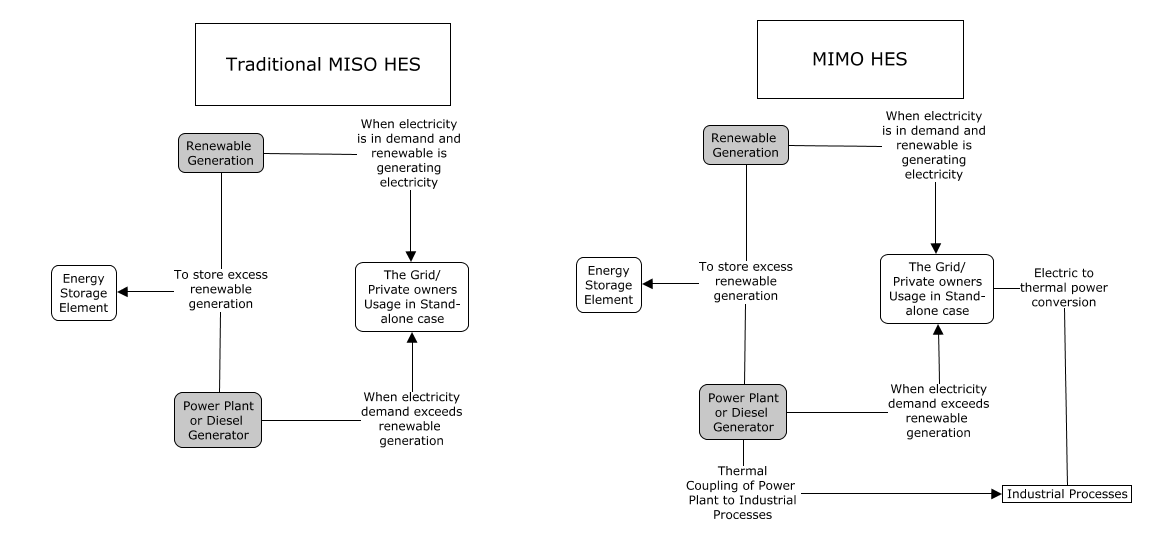
\includegraphics[width=\textwidth]{MISO_MIMO.png}
\caption{\small \sl This figure compares the MISO and MIMO configurations, demonstrating the differences between traditional \ac{hes} that are focused on generating reliable electricity and non-traditional \ac{hes}, which have the added objective of generating an additional product.  While many of the elements are the same, the MIMO system includes an Industrial Process  that is either thermally or electrically coupled.}
\label{MIMO_MISO}
\end{figure*}

\section{Nuclear Renewable Hybrid Energy Systems}
\ac{nrhess} are defined by Bragg-Sitton et al. (2014) as the

\begin{quotation}
"tighter coupling of nuclear and renewable energy sources in a manner that better optimizes energy use for the combined electricity, industrial manufacturing, and transportation sectors capable of apportioning thermal electrical energy to first meet the grid demand (with appropriate power conversion systems), then utilizing excess thermal and, in some cases, electrical energy to drive a process that results in an additional product \cite {Bragg-Sitton2014}".
\end{quotation} The benefits to the participants of the \ac{nrhes} that co-locate their facilities include minimizing system wide costs to the \ac{nrhes} while increasing economic resilience by diversifying both the means of generating energy as well as the products produced. For example, if natural gas prices increase, the \ac{nrhes} could rely less on the natural gas plant and put more focus on storage.  If short-term electricity prices are negative, the energy produced by the \ac{nrhes} can be diverted to the industrial process.

The additional industrial processes possible to couple in a \ac{nrhes} include, but are not limited to: heat added to synthetic fuel upgrading, heat for titanium dioxide production, heat and/or electricity for desalinated water, heat and/or electricity for hydrogen production, heat for aluminum production or recycling, and thermal storage through heat pumps \cite{Bienvenue2015}.  Current uses of thermally coupled \ac{npps} are for district heating and heat for papermills \cite{Verfondern}. The \ac{npp} distributes the energy it generates between the grid and the industrial process to maximize profit. The system can allocate energy based on the market value of each of the multiple outputs produced. In the case of a NPP coupled with a desalination plant, for example, if the price of electricity is low, more thermal and/or electric energy can be diverted to generate more clean water at a higher profit \cite {Chen2016}. The costs of operating a dynamic system, such as the case with a \ac{nrhes}, include additional wear and tear, decreased thermal efficiency  due to variability, and increased complexity of operations  \cite{Garcia2013}. The total net costs of the system, such as meeting regulatory expectations, have yet to be determined.

\section{Ongoing Modeling Research}
There have been no physical demonstrations to date of \ac{nrhes}. Research has largely focused on computational modeling to determine the feasibility and optimization of coupling elements \cite{Rabiti2015, Shropshire2012}. The literature review revealed that much of the work on \ac{nrhess} is in the design and analysis stage \cite{Epiney2016, Shropshire2012}. Research has focused on developing models that can dynamically simulate the contributions of variable energy sources, the constraints of flexibly operating electricity demand, and thermal/electrical power demands for various industrial processes. The models focus on answering questions regarding minimizing the cost of electricity and ensuring profitability for each of the components comprising the \ac{nrhes}. In order to move forward with development of any \ac{nrhes}, such systems must demonstrate that they can be profitable and can reliably respond to variable electricity production and demand \cite{Rabiti2015}.

An ongoing effort at \ac{inl}, \ac{anl}, and \ac{ornl} focuses on modeling a generic \ac{nrhes} to optimize the size of the components as well as the overall functioning of the system. The generic model will test the economic viability of \ac{nrhess} to determine if future development should be pursued. The industrial plant combines a \ac{npp}, a wind farm, a natural gas power plant, a battery, and a high temperature steam electrolysis hydrogen production facility. More component models will be developed in the future that can compare various industrial customers \cite{Harrison2016}. The chosen renewable source, a wind farm, models a highly stochastic system due to the unpredictable nature of wind generation \cite{Chen2016_wind}. The model optimizes the sizes of the \ac{npp}, the natural gas plant, and the battery. The model performs two optimizations, the first on the size of the components and the second optimizing the functioning of the system to minimize costs \cite{redfoot_rabiti_2018}. The objective is to choose the \ac{nrhes} configuration that minimizes costs while meeting set emissions and grid reliability expectations.

\section{Computational Tools}
\ac{nrhes} sit in an interesting location in computational modeling. There are many tools to model and optimize non-nuclear \ac{hes} (HOMER, Hybrid2, SOLSIM, SOMES, ARES, RAPSIM, HOGA) \cite {Bernal-Agustin2009}. These programs calculate mass flow, electricity output, and the possible output of another product, such as hydrogen. Modelica and Excel, while neither specifically HES nor \ac{nrhes} tools, have been used to model both nuclear and non-nuclear \ac{hes}s \cite{Shropshire2012, Chen2016, Binder2014, Garcia2015, Epiney2016}. HES tools have typically been developed for microgrid standalone systems. The main challenges to applying HES systems to a \ac{nrhes} are the scale of the system being modeled and fluctuating grid demand.

\section{\ac{nrhes} Models}
Selecting a tool to model a \ac{nrhes} requires understanding what characteristics a model must possess in order to provide accurate information. For example, as discussed below, it is important for a \ac{nrhes} model to incorporate the dynamic nature of the system in order to include losses from the changes in the system. Rabiti et al. (2015) discusses the important elements of a \ac{nrhes} computational model in detail, describing the basic requirements of the software as a

\begin{quotation}
"computational representation of the thermal, mechanical, chemical, and electrical processes in the systems as process units, reactors, manufacturing plants, and energy delivery (to the appropriate point of interface with the market transaction, such as an electricity bus, or a product depot or distribution terminal where a commodity price is established)\cite{Rabiti2015}."
\end{quotation}

The model in development by the national laboratories combines \ac{raven} for the stochastic and statistical aspects of the system, such as generating synthetic wind data based on actual wind data and optimizing the systems, with Modelica for modeling the various components in the \ac{nrhes}.

\subsection{Modelica}
Modelica is a widely used open source language for modeling large and complex systems composed of smaller component models. It is particularly suited for modeling dynamic systems. Modelica has powerful libraries, such as Thermopower, that include the thermohydraulic modeling tools required for modeling mass flows in energy systems \cite{Binder2014}. The language is well-maintained, giving it the added benefits of having up-to-date documentation and a community that can provide support. Typically Modelica is run on the Dymola developer environment, a private tool developed by the creator of Modelica, Dr. Hilding Elmquist. Another option for running the Modelica language is the open source OpenModelica environment.

A Modelica HES model developed in Binder et. al. (2014) includes a nuclear reactor, two steam cycles, a chemical plant, and an electrical component \cite{Binder2014}. The products of the system modeled are synthetic fuel and electricity. The model includes the ramp up stage when the reactor initially starts or is increasing from a lower load. The steam generator connected to the NPP determines which of its turbines to use depending on electricity demand, the 60\% turbine, the 30\% turbine, or the 15\% turbine, which can be used in unison. A pressure relief valve releases excess energy unused by the turbines. The wind generation is modeled using the Western Wind dataset from the \ac{nrel} for an unspecified region in Idaho. Each component in the model was tested individually before being combined. Using the individual component models, verifications were made for the system as a whole. As demonstrated in Binder et al. (2014), running a model of a \ac{nrhes} in Modelica requires a control algorithm, a differential equation that controls how the dynamic system allocates heat. The profitability control algorithm can be adjusted to incorporate varying parameters such as the price of electricity or the cost of natural gas. The study concluded that Modelica, due to its ability to evaluate control algorithms, is an effective tool for dynamically modeling a HES. As a tool that is optimized for large dynamic systems, Modelica has been used more than any other tool to model \ac{nrhess} at this point.

\subsection{RAVEN}


The RAVEN tool was initially built for probabilistic risk assessment. RAVEN, as a probabilistic tool, can do parametric and stochastic analyses of systems\cite{RabitiRAVEN}. For \ac{nrhess}, RAVEN is used to run different wind energy generation paths in order to generate a statistically fair representation of how renewables, in this case wind power, would likely function over any given week. RAVEN can be used to produce data representing the most generic seasonal wind generation over a week. A typical week can be extrapolated to represent a given season. The process can be repeated over the different seasons, which can be extrapolated to represent a year. Using synthetic generated data instead of historic data avoids the critique that the model only represents past behavior and is thus not applicable to future trends \cite{redfoot_epiney_2016}. RAVEN can also be used to determine high-risk time series samples to ensure that high risk scenarios are accounted for in the study. RAVEN can also do probabilistic assessments such as loss of load probability and sensitivity to uncertainty analysis.

Any future modeling efforts for a \ac{nrhess} would benefit from complimenting the ongoing modeling effort. Currently, all of the physics models for the \ac{nrhes} are built in Modelica. To benefit from the work already done, any additional software would need to be able to easily communicate with the Modelica modeling language.  The model would benefit from a tool that would communicate with other chemical and utility standard physics modeling tools. Future work would benefit from coupling with other physics modeling tools, allowing groups to take advantage of the existing infrastructure while using their physics model of choice.

\subsection{Distinct Capabilities}
There are certain characteristics of a physical \ac{nrhes} which a computational model would need to reasonably assess the system as a whole. These are summarized at the end of the chapter in Table \ref{table:1} which demonstrates the functions most commonly incorporated in a model. The following discussion details the extensive work that has been done determine why dynamisticity is important to modeling a \ac{nrhes}.

In Garcia et. al. (2013) and Du et. al. (2014), a dynamic approach to modeling \ac{hes} is applied in order to appropriately address the impacts of flexible operation of the system due to variable renewable generation \cite{Garcia2013, Du2014}. In Du et. al. (2014), two optimization problems are addressed: the first minimizes variability in the HES through optimizing components of the HES system, and the second imposes operating and capital costs on the design variables. Garcia et. al. (2013) has a two-part series. The first applies and analyzes performance of a dynamic approach to modeling some of the physical components of a traditional and an advanced MIMO HES. The second paper focuses on economic effects using a dynamic approach, as opposed to time series or statistical analysis. Overall, both parts of the series focus on how a dynamic approach better models the high level of variability of a HES for output generation and profitability maximization \cite{Garcia2013}. The costs of operating in a flexible manner, dynamically allocating resources between multiple coupled systems, are substantial enough to require a simulation that precisely models the variability of the system \cite{Garcia2013, Shropshire2011, Locatelli2015}. The dynamic modeling at this point focuses on the dynamic transfer of energy to different sources, and how this impacts the system economics and grid reliability. The physical impacts of the grid system have not yet been included in the most developed \ac{nrhes} simulation, the national laboratory model \cite{Harrison2016}.  The dynamic allocation of the heat and electricity, which depend on the renewable generation and the grid demand is an essential characteristic of a \ac{nrhes}.  Including factors such as how quickly the \ac{nrhes} will be able to switch between providing energy to the industrial facility and the grid will impact determining the economic and physical values of the model.

\section{Small Modular Reactors}
For completeness, the use of \ac{smrs} both as tools for load following and as sources of process heat must be addressed. SMRs are generally defined as nuclear reactors under 300 MWe. SMR designs, such as that in development by NuScale, combine multiple small reactor modules. Multiple SMRs in combination are a promising possibility for \ac{nrhess}.  With multiple reactors, individual modules can be assigned to meet the industrial process energy demand, with others solely used for electricity generation. Furthermore, as electricity demand grows, additional modules can be added to the industrial park. Multiple SMRs have a clear means of load following, simply by shutting down those reactors whose energy output is not required due to seasonal shifts and other demand factors. The modularity of the SMRs allows greater flexibility in the design of the industrial park.  Locatelli (2015) discusses the technical and economic feasibility of load following using multiple SMRs, applying the excess energy toward generating algae-biofuel and desalinated water \cite{Locatelli2015}. He discusses the benefits as well as drawbacks of a \cite{nrhes} that includes a thermal desalination process. A desalination plant has the benefits of switching between a latent and producing state and generating a product that is readily stored. The main drawback is poor water quality and output level when the desalination unit restarts. In general, SMRs have multiple means of adjusting their electricity output to the grid including coupling with an industrial process.

The NuScale reactor, with proposed construction starting in 2025 at INL, has motivated research into different methods of flexibly operating the amount of electricity sent to the grid \cite{Ingersoll2014, Ingersoll2015, Ingersoll2016, Ingersoll2014_1}. The NuScale reactor design, as can be seen in the figure below, combines twelve small pressurized water reactors into one large pool of water.  Each of the reactors is rated at 50 MWe, generating a combined 600 MWe. The NuScale reactor has been evaluated to thermally couple with oil refining processes, multiple desalination techniques, as well as hydrogen production \cite{Ingersoll2014}. Aside from thermally coupling and rerouting the energy from electricity generation to process heat applications, the NuScale reactors have furthermore been evaluated for loosely coupling with the Horse Butte Wind Farm in nearby Idaho Falls \cite{Ingersoll2015}.  The NuScale plant has multiple approaches to meet the changing electricity demanded by the grid, which NuScale designates as NuFollow \cite{Ingersoll2015}.  The NuScale plant can take down one or more of the low power reactors, changing the power output of one or more modules for shorter changes in the grid demand due to changes in wind output, and sending the heat generated by the reactor straight to the condenser bypassing the power generating turbine cycle.
\begin{figure*}[h!]
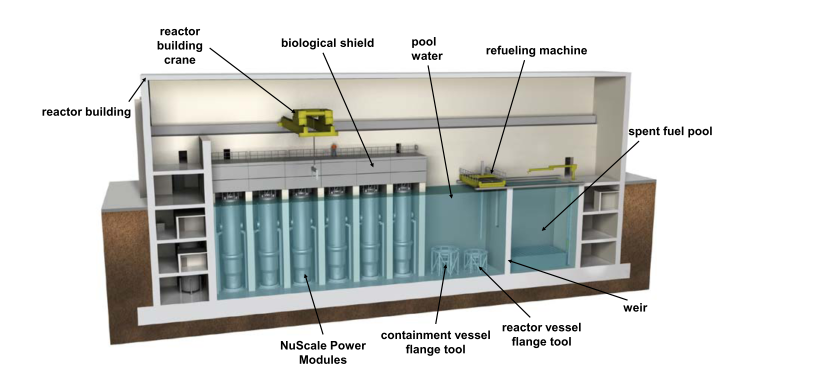
\includegraphics[width=\textwidth]{NuScale_cutaway.PNG}
\caption{\small \sl This figure from \cite{Ingersoll2014} displays the design of half of the NuScale plant. Six of the reactor modules can be seen in the cooling pool along with the crane which inserts and removes the modules.}
\label{nuscale}
\end{figure*}
\subsection{Other Research on \ac{nrhes} Models}
Many more studies on HESs and \ac{nrhess} incorporate economic and technical modeling, but the essential characteristics of ability to model a dynamic and stochastic system have been covered. For completeness of the state of the art research on \ac{nrhess}, some of the other relevant studies include:
\begin{itemize}
\item Shropshire et. al. (2012) does not focus on HES, but discusses how different models of flexible and small modular reactors could integrate into the European energy market with growing renewable generation, thus fulfilling the growing need for flexibility and load following in other electricity suppliers \cite{Shropshire2012}.
\item Shropshire et. al. (2011) develops target cost estimates for reactors given certain economic environments based on competing technology energy costs \cite{Shropshire2011}.
\item OECD-NEA (2011), Nuclear Energy Agency Organisation for Economic Co-operation and Development, presents an overview of the capability of implemented newer and older \ac{npp}s to load follow \cite{Nuclear2011}.
\item Baker (2016) analyzes the \ac{lcoe} as the \ac{fom} and the role of battery storage to evaluate different \ac{nrhess} scenarios \cite{Baker2016}
\item Kazimi et al. (2009) produces a preliminary dynamic analysis of two \ac{nrhess} that have high levels of renewable energy generation and multiple outputs from the system. The study concludes that \ac{nrhess} could lead to optimized energy use, reduced carbon, favorable economic performance, and flexible operation time \cite{Kazimi}.
\item Forsberg et. al. (2009) discusses using nuclear power to create more liquid transportation fuels from biomass and fossil fuel sources \cite{Forsberg2009}.
\item There have also been two regional modeling studies conducted for Texas and Arizona focused on including regional characteristics to determine the renewable used and the industrial process\cite{Garcia2015}.
\end{itemize}
Table \ref{table:1} displays the characteristics routinely described as necessary to model a \ac{nrhes} along with their citations.

\begin{table}[h!]
\centering
\caption{References for Each \ac{nrhes} Characteristic}
\begin{tabular}{ ||c | c|| }
 \hline
 \ac{nrhes} Characteristic & Paper \\ [0.5ex]
 \hline \hline
 Dynamic & \cite{Garcia2013, Du2014, Kazimi, Garcia2016}\\
 \hline
 Sensitivity Analysis & \cite{Shropshire2011, Rehman2010, Adaramola2014, Chen2016}\\
 \hline
 Optimization of components & \cite{Chen2016,Ozcan2016, Forsberg2009,Garcia2015,Aumeier2011}\\
 \hline
 Stochastic Model of Renewables & \cite{Rabiti2015, Garcia2016,Locatelli2015}\\
 \hline
 Grid Demand model & \cite{Forsberg2013, Garcia2016,Garcia2013,Ruth2014,Chen2016}\\
 \hline
  Economic FOMs & \cite{Garcia2016,Chen2016,Rabiti2015,Epiney2016,Bragg-Sitton2014}\\
 \hline
\end{tabular}
\label{table:1}
\end{table}

The six characteristics included in Table \ref{table:1} are those likely necessary for a \ac{nrhes} model to be reasonably accurate.  Each of the characteristics has been included in previous studies, and thus has some already proposed approaches.  The characteristics can be studied in greater detail in order to determine if they satisfactorily model the system.
